
\begin{center}
\Huge
	Trigonometriske ligninger
\end{center}
\section*{Trigonometriske ligninger}
\stepcounter{section}

Vi ønsker at kunne bestemme eksakte løsninger til trigonometriske ligninger - altså ligninger, hvor der indgår $\cos$, $\sin$ og $\tan$. For at kunne bestemme sådanne løsninger eksakt, vil de særlige vinkler, vi tidligere arbejdede med, altså heltalsmultiplum af $\frac{\pi}{6}$ og $\frac{\pi}{4}$ være særligt centrale. Vi får derfor brug for enhedscirklen på Figur \ref{fig:enhed}
\begin{figure}[H]
	\centering
	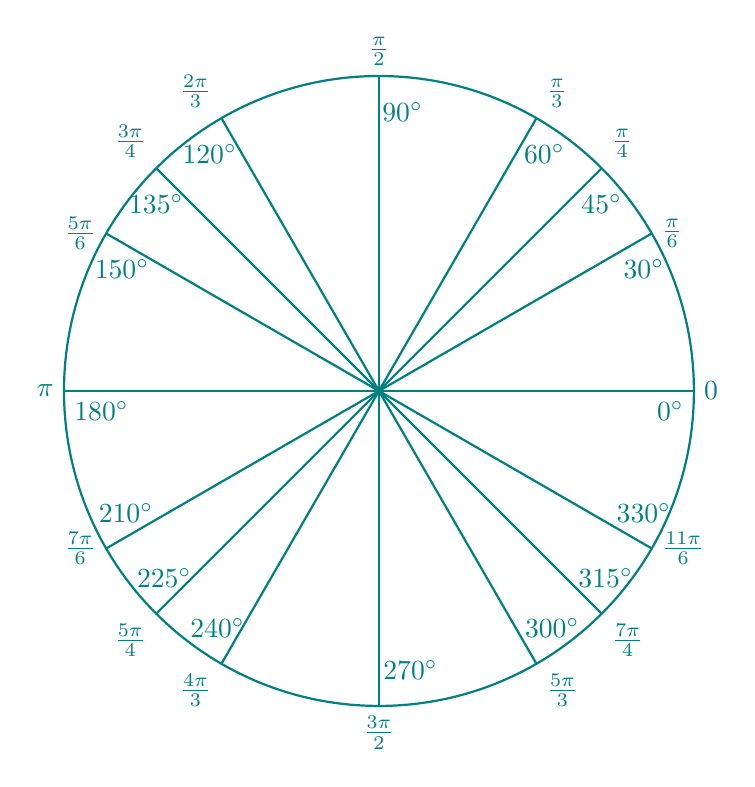
\begin{tikzpicture}
		\draw[thick, color = teal] (0,0) circle (4cm);
		\draw[thick, color = teal] (0,0) -- ({4*cos(0)},{4*sin(0)})
		node[pos = 1, anchor = north east] {$0^\circ$}
		node[pos = 1, anchor = west] {0};
		\draw[thick, color = teal] (0,0) -- ({4*cos(30)},{4*sin(30)})
		node[pos = 1, anchor = north, yshift = -0.2cm, xshift = -0.1cm] {$30^\circ$}
		node[pos = 1, anchor = west] {$\frac{\pi}{6}$};
		\draw[thick, color = teal] (0,0) -- ({4*cos(45)},{4*sin(45)})
		node[pos = 1, anchor = north, yshift = -0.2cm, xshift = -0cm] {$45^\circ$}
		node[pos = 1, anchor = south west] {$\frac{\pi}{4}$};
		\draw[thick, color = teal] (0,0) -- ({4*cos(60)},{4*sin(60)})
		node[pos = 1, anchor = north, yshift = -0.2cm, xshift = 0.1cm] {$60^\circ$}
		node[pos = 1, anchor = south west] {$\frac{\pi}{3}$};
		\draw[thick, color = teal] (0,0) -- ({4*cos(90)},{4*sin(90)})
		node[pos = 1, anchor = north, yshift = -0.2cm, xshift = 0.3cm] {$90^\circ$}
		node[pos = 1, anchor = south] {$\frac{\pi}{2}$};
		\draw[thick, color = teal] (0,0) -- ({4*cos(120)},{4*sin(120)})
		node[pos = 1, anchor = north, yshift = -0.2cm, xshift = -0.15cm] {$120^\circ$}
		node[pos = 1, anchor = south east] {$\frac{2\pi}{3}$};
		\draw[thick, color = teal] (0,0) -- ({4*cos(135)},{4*sin(135)})
		node[pos = 1, anchor = north, yshift = -0.2cm, xshift = -0cm] {$135^\circ$}
		node[pos = 1, anchor = south east] {$\frac{3\pi}{4}$};
		\draw[thick, color = teal] (0,0) -- ({4*cos(150)},{4*sin(150)})
		node[pos = 1, anchor = north, yshift = -0.2cm, xshift = 0.2cm] {$150^\circ$}
		node[pos = 1, anchor = east] {$\frac{5\pi}{6}$};
		\draw[thick, color = teal] (0,0) -- ({4*cos(180)},{4*sin(180)})
		node[pos = 1, anchor = north west] {$180^\circ$}
		node[pos = 1, anchor = east] {$\pi$};
		\draw[thick, color = teal] (0,0) -- ({4*cos(210)},{4*sin(210)})
		node[pos = 1, anchor = south, yshift = 0.2cm, xshift = 0.25cm] {$210^\circ$}
		node[pos = 1, anchor = east] {$\frac{7\pi}{6}$};
		\draw[thick, color = teal] (0,0) -- ({4*cos(225)},{4*sin(225)})
		node[pos = 1, anchor = south, yshift = 0.2cm, xshift = 0.1cm] {$225^\circ$}
		node[pos = 1, anchor = north east] {$\frac{5\pi}{4}$};
		\draw[thick, color = teal] (0,0) -- ({4*cos(240)},{4*sin(240)})
		node[pos = 1, anchor = south, yshift = 0.2cm, xshift = -0.05cm] {$240^\circ$}
		node[pos = 1, anchor = north east] {$\frac{4\pi}{3}$};
		\draw[thick, color = teal] (0,0) -- ({4*cos(270)},{4*sin(270)})
		node[pos = 1, anchor = south, yshift = 0.2cm, xshift = 0.4cm] {$270^\circ$}
		node[pos = 1, anchor = north] {$\frac{3\pi}{2}$};
		\draw[thick, color = teal] (0,0) -- ({4*cos(300)},{4*sin(300)})
		node[pos = 1, anchor = south, yshift = 0.2cm, xshift = 0.2cm] {$300^\circ$}
		node[pos = 1, anchor = north west] {$\frac{5\pi}{3}$};
		\draw[thick, color = teal] (0,0) -- ({4*cos(315)},{4*sin(315)})
		node[pos = 1, anchor = south, yshift = 0.2cm, xshift = 0.05cm] {$315^\circ$}
		node[pos = 1, anchor = north west] {$\frac{7\pi}{4}$};
		\draw[thick, color = teal] (0,0) -- ({4*cos(330)},{4*sin(330)})
		node[pos = 1, anchor = south, yshift = 0.2cm, xshift = -0.1cm] {$330^\circ$}
		node[pos = 1, anchor = west] {$\frac{11\pi}{6}$};
	\end{tikzpicture}
	\caption{Enhedscirklen med udvalgte vigtige vinkler.}
	\label{fig:enhed}
\end{figure}
Vi skal også bruge Tabel \ref{tab:trig} over vigtige værdier for cos, sin og tan for netop disse vinkler.
\begin{table}[H]
	\centering
	\rowcolors{1}{SeaGreen!20}{Melon!20}
	\begin{tabular}{cccccc}
		$\theta$ & 0 & $\frac{\pi}{6}$ & $\frac{\pi}{4}$ & $\frac{\pi}{3}$ & $\frac{\pi}{2}$ \\
		$\cos(\theta)$ & 1 &  $\frac{\sqrt{3}}{2}$ & $\frac{\sqrt{2}}{2}$ & $\frac{1}{2}$ & 0 \\
		$\sin(\theta)$ & 0 & $\frac{1}{2}$ & $\frac{\sqrt{2}}{2}$ &  $\frac{\sqrt{3}}{2}$ & 1 \\
		$\tan(\theta)$ & 0 &  $\frac{\sqrt{3}}{3}$ & 1 & $\sqrt{3}$ & 
	\end{tabular}
	\caption{Vigtige funktionsværdier for cos, sin og tan.}
	\label{tab:trig}
\end{table}
Lad os betragte et eksempel.
\begin{exa}
	Vi ønsker at løse $2\sin(x)^2 - \sin(x) = 0$ på intervallet $0\leq x \leq 2\pi$. Vi sætter $y = \sin(x)$ og får
	\begin{align*}
		2y^2 - y = 0 \ &\Leftrightarrow \ y(2y - 1) = 0.
	\end{align*}
	Vi får derfor, at $y = 0$ eller $y = 0.5$, og derfor, at $\sin(x)=0$ eller $\sin(x)=0.5$. Vi bruger nu
	 Tabel \ref{tab:trig} samt Figur \ref{fig:enhed} og får, at $x = 0$ eller $x = \pi$, hvis $\sin(x) = 0$. 
	 Vi får tilmed, at $x = \frac{\pi}{6}$ eller $\frac{5\pi}{6}$, hvis $\sin(x) = 0.5.$ Løsningerne til ligningen er
	 derfor 
	 \begin{align*}
	 	x= 0, x = \pi, x = \frac{\pi}{6}, x = \frac{5\pi}{6}
	 \end{align*}
\end{exa}

\subsection*{Opgave 1}

Løs følgende ligninger for $0 \leq x \leq 2\pi$.
\begin{align*}
	&1) \  \cos(x) - 1 = 0   &&2) \  2\cos(x) - 1 = 0   &&3) \ 1 - \tan(x) = 0    \\
	&4) \  2\sin(x) = \sqrt{2}   &&5) \   9\tan(x)^2 = 3   &&6) \  \cos(x)^2 - \frac{1}{2} = 0   \\
	&7) \  2\sin(x) +\sqrt{3} = 0  &&8) \  \tan(x)^2 - 1 = 0    &&9) \ \cos(x)^2 + \frac{1}{4} - \cos(x) = 0    \\
\end{align*}

\subsection*{Opgave 2}

Løs følgende ligninger for $0 \leq x \leq 2\pi$. 

\begin{align*}
	&1) \  \sin\left( x - \frac{\pi}{2}\right) = 0  &&2) \  \cos\left( x + \frac{\pi}{3}\right) = \frac{1}{2}  
	 &&3) \tan\left( x - \frac{\pi}{4}\right) = 1  \\
	&4) \ 3\tan\left( x - \pi \right) = -\sqrt{3}   &&5) \   \cos\left( x - \frac{5\pi}{6}\right) = \frac{\sqrt{2}}{2}   &&6) \ \sin\left( 2x - \frac{11\pi}{6}\right) = -1   \\
\end{align*}

\subsection*{Opgave 3}
Løs følgende ligninger for $0 \leq x \leq 2\pi$.
\begin{align*}
	&1) \ \cos(x)^2 - \cos(x) = 0    &&2) \  \sin(x)^2 + \frac{1}{2}\sin(x) = 0    \\
	&3) \ \cos(x)^2 -\frac{1}{2}\cos(x) = \frac{1}{2}   &&4) \  \tan(x)^2 -\frac{2\sqrt{3}}{3}y+\frac{1}{3} = 0 \\
	&5) \  2\sin(x)^2 - (\sqrt{3}+\sqrt{2})\sin(x) + \sqrt{6} = 0     &&6) \  \tan(x)^2 - 1 = 0    \\
\end{align*}